%!TEX root = Manuscript.tex

\chapter{Use case of matching guided by 2D similarity transformation}
\label{chap:appendix3}
In this section we compare the performance of \textit{state-of-the-art} matching methods: (1) SIFT and (2) SuperGlue, as well as our matching strategy: (3) SIFT under the guidance of 2D similarity transformation model followed by RANSAC to remove outliers. 
\par
For each keypoint in the master image, our strategy uses 2D similarity transformation model to predict a location in the secondary image and search only its neighborhood (30 pixel in our experiment) to reduce ambiguity.\\
\section{Dataset}
This dataset consists of several archival aerial images taken at 1945, provided by the National Survey of Iceland. The images are over a snow-covered area with low contrast. In Figure~\ref{SnowData} we displayed 6 consecutive images in the same flight strip, with snow-covered area gradually expanding. We chose the most challenging image pair (i.e. image 5 and 6, as they are fully snow-covered with very limited context) for testing. Their common zone is labeled with red rectangles. The size of both images is 14014$\times$14009 pixels.\\
For generating the 2D similarity transformation parameters that are required for our matching strategy, we manually measure only 1 match to estimate the translation, as they are images taken at the same flight stripe, the scale and rotation are approximately equal to 1 and 0, respectively.\\
%Figure~\ref{Matchresult} demonstrated the matching result of SIFT, SuperGlue and our matching strategy.\\
\begin{figure*}[htbp]
	\begin{center}
		\subfigure[Image 1]{
			\begin{minipage}[t]{0.31\linewidth}
				\centering
				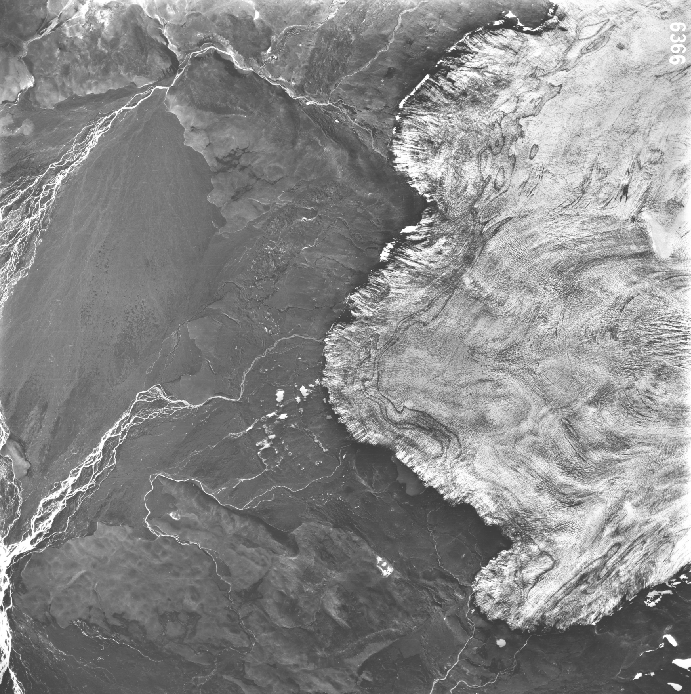
\includegraphics[width=4.3cm]{images/appendix3/3-6366_crp_8Bits_Zoom8.png}
			\end{minipage}%
		}
		\subfigure[Image 2]{
	\begin{minipage}[t]{0.31\linewidth}
		\centering
		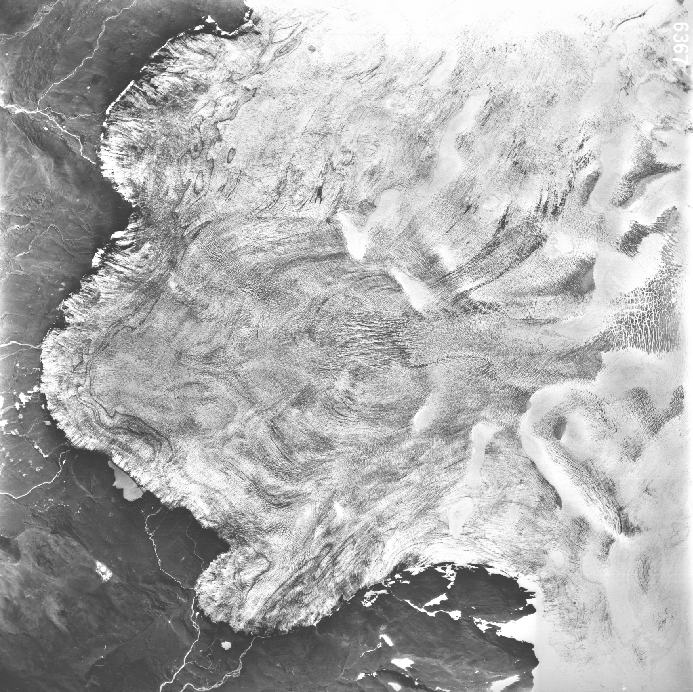
\includegraphics[width=4.3cm]{images/appendix3/3-6367_crp_8Bits_Zoom8.png}
	\end{minipage}%
}
		\subfigure[Image 3]{
	\begin{minipage}[t]{0.31\linewidth}
		\centering
		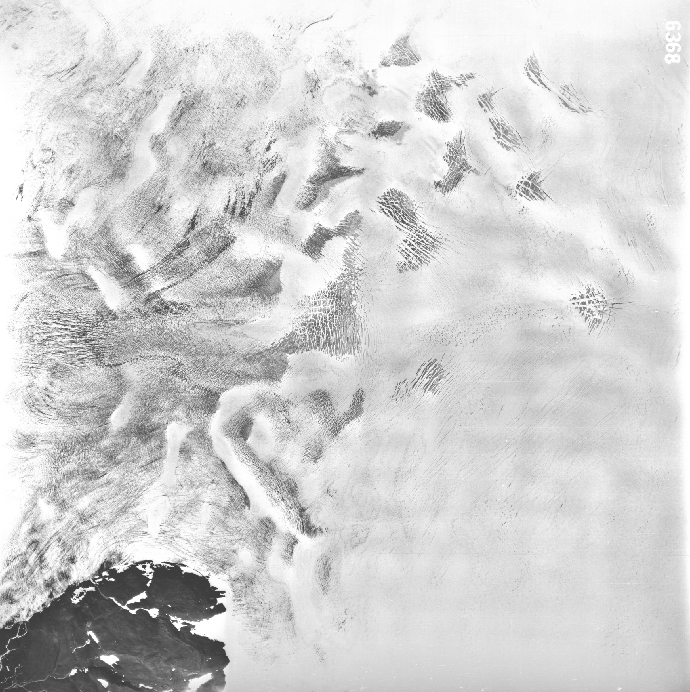
\includegraphics[width=4.3cm]{images/appendix3/3-6368_crp_8Bits_Zoom8.png}
	\end{minipage}%
}
		\subfigure[Image 4]{
	\begin{minipage}[t]{0.31\linewidth}
		\centering
		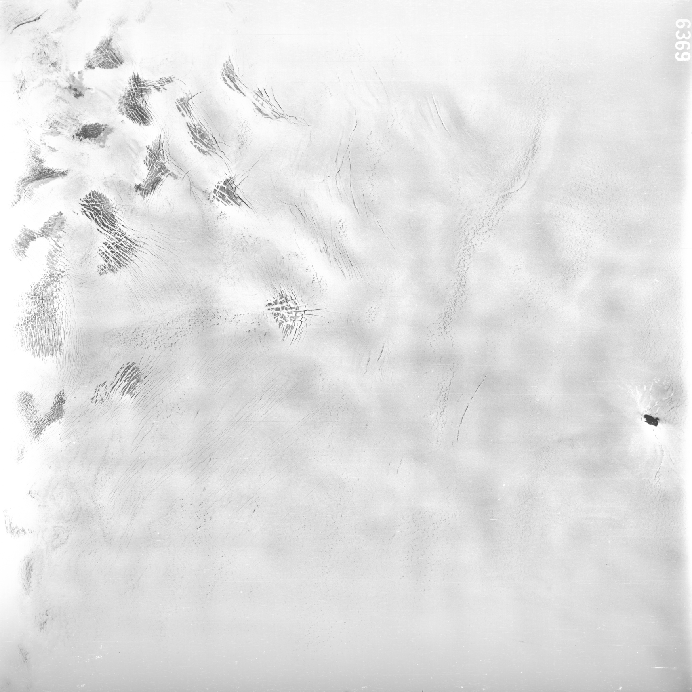
\includegraphics[width=4.3cm]{images/appendix3/3-6369_crp_8Bits_Zoom8.png}
	\end{minipage}%
}
\subfigure[Image 5]{
	\begin{minipage}[t]{0.31\linewidth}
		\centering
		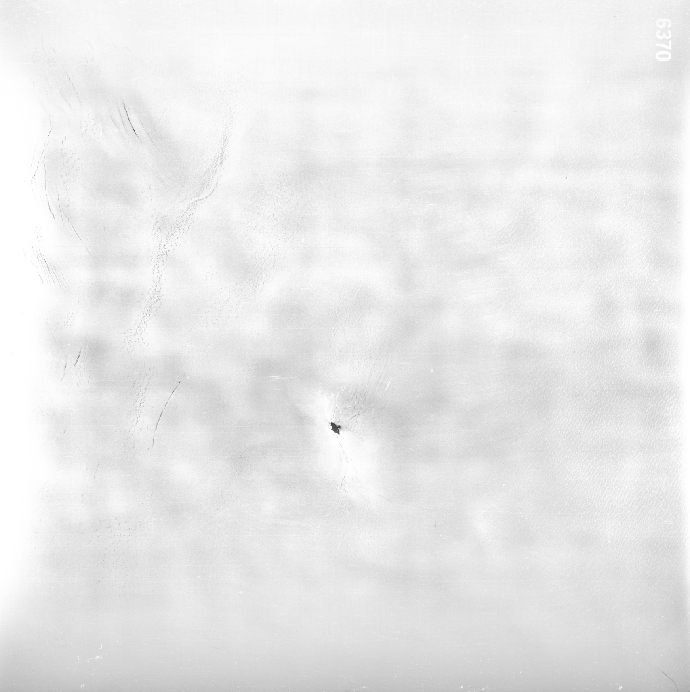
\includegraphics[width=4.3cm]{images/appendix3/3-6370_crp_8Bits_Zoom8.png}
	\end{minipage}%
}
\subfigure[Image 6]{
	\begin{minipage}[t]{0.31\linewidth}
		\centering
		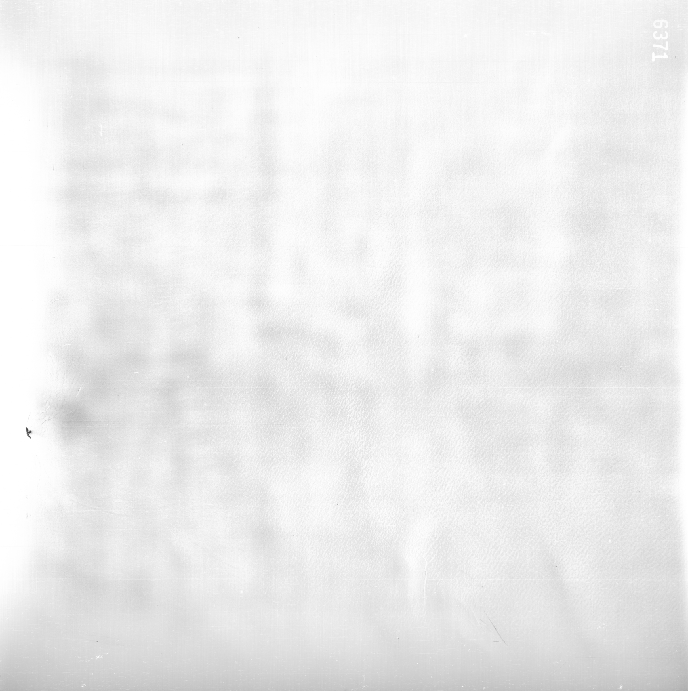
\includegraphics[width=4.3cm]{images/appendix3/3-6371_crp_8Bits_Zoom8.png}
	\end{minipage}%
}
		\caption{Images demonstration of the dataset. (a-f) are consecutive images in the same flight line with a wide range of area covered with snow. (e) and (f) are chosen as the testing image pair, whose common zone is pointed out as red rectangles.}
		\label{SnowData}
	\end{center}
\end{figure*} 

\section{Result}
Figure~\ref{Matchresult} demonstrated the matching result of SIFT, SuperGlue and our matching strategy. As can be seen, SIFT and SuperGlue failed to found any correct matches, while our strategy obtained a large number of good matches with negligible manual labor.
\begin{figure*}[htbp]
	\begin{center}
		\subfigure[SIFT]{
			\begin{minipage}[t]{0.48\linewidth}
				\centering
				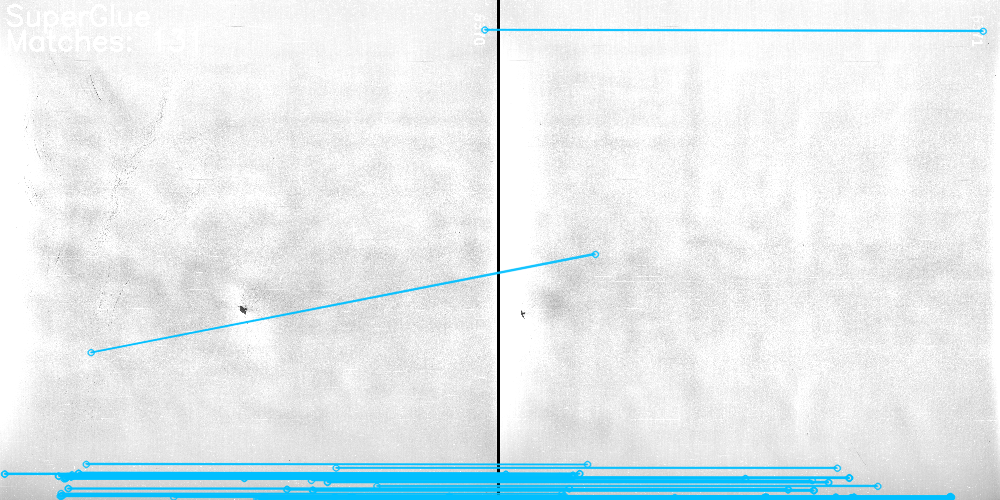
\includegraphics[width=6.3cm]{images/appendix3/Homol-TXT_3-6370_crp_8Bits_3-6371_crp_8Bits.png}
			\end{minipage}%
		}
		\subfigure[SuperGlue]{
			\begin{minipage}[t]{0.48\linewidth}
				\centering
				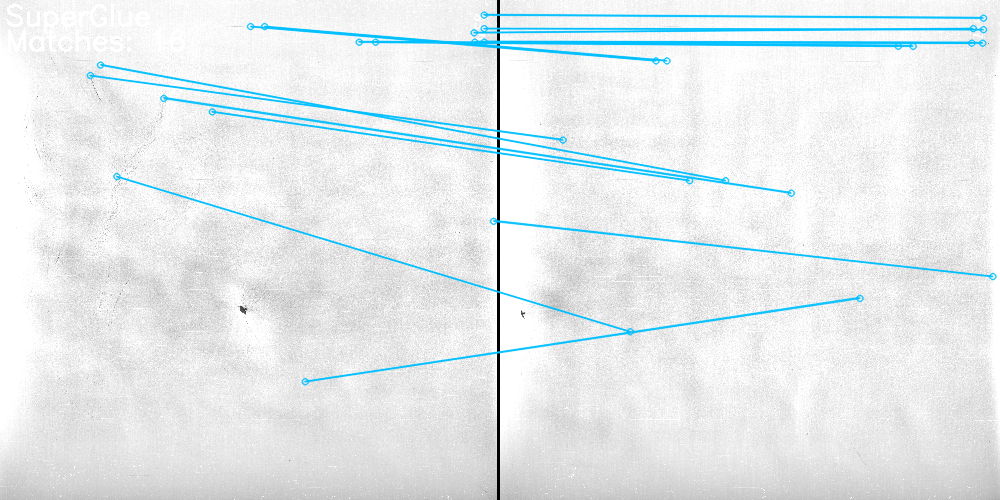
\includegraphics[width=6.3cm]{images/appendix3/Homol-SuperGlue_3-6370_crp_8Bits_3-6371_crp_8Bits.png}
			\end{minipage}%
		}
		\subfigure[Guided SIFT]{
			\begin{minipage}[t]{1\linewidth}
				\centering
				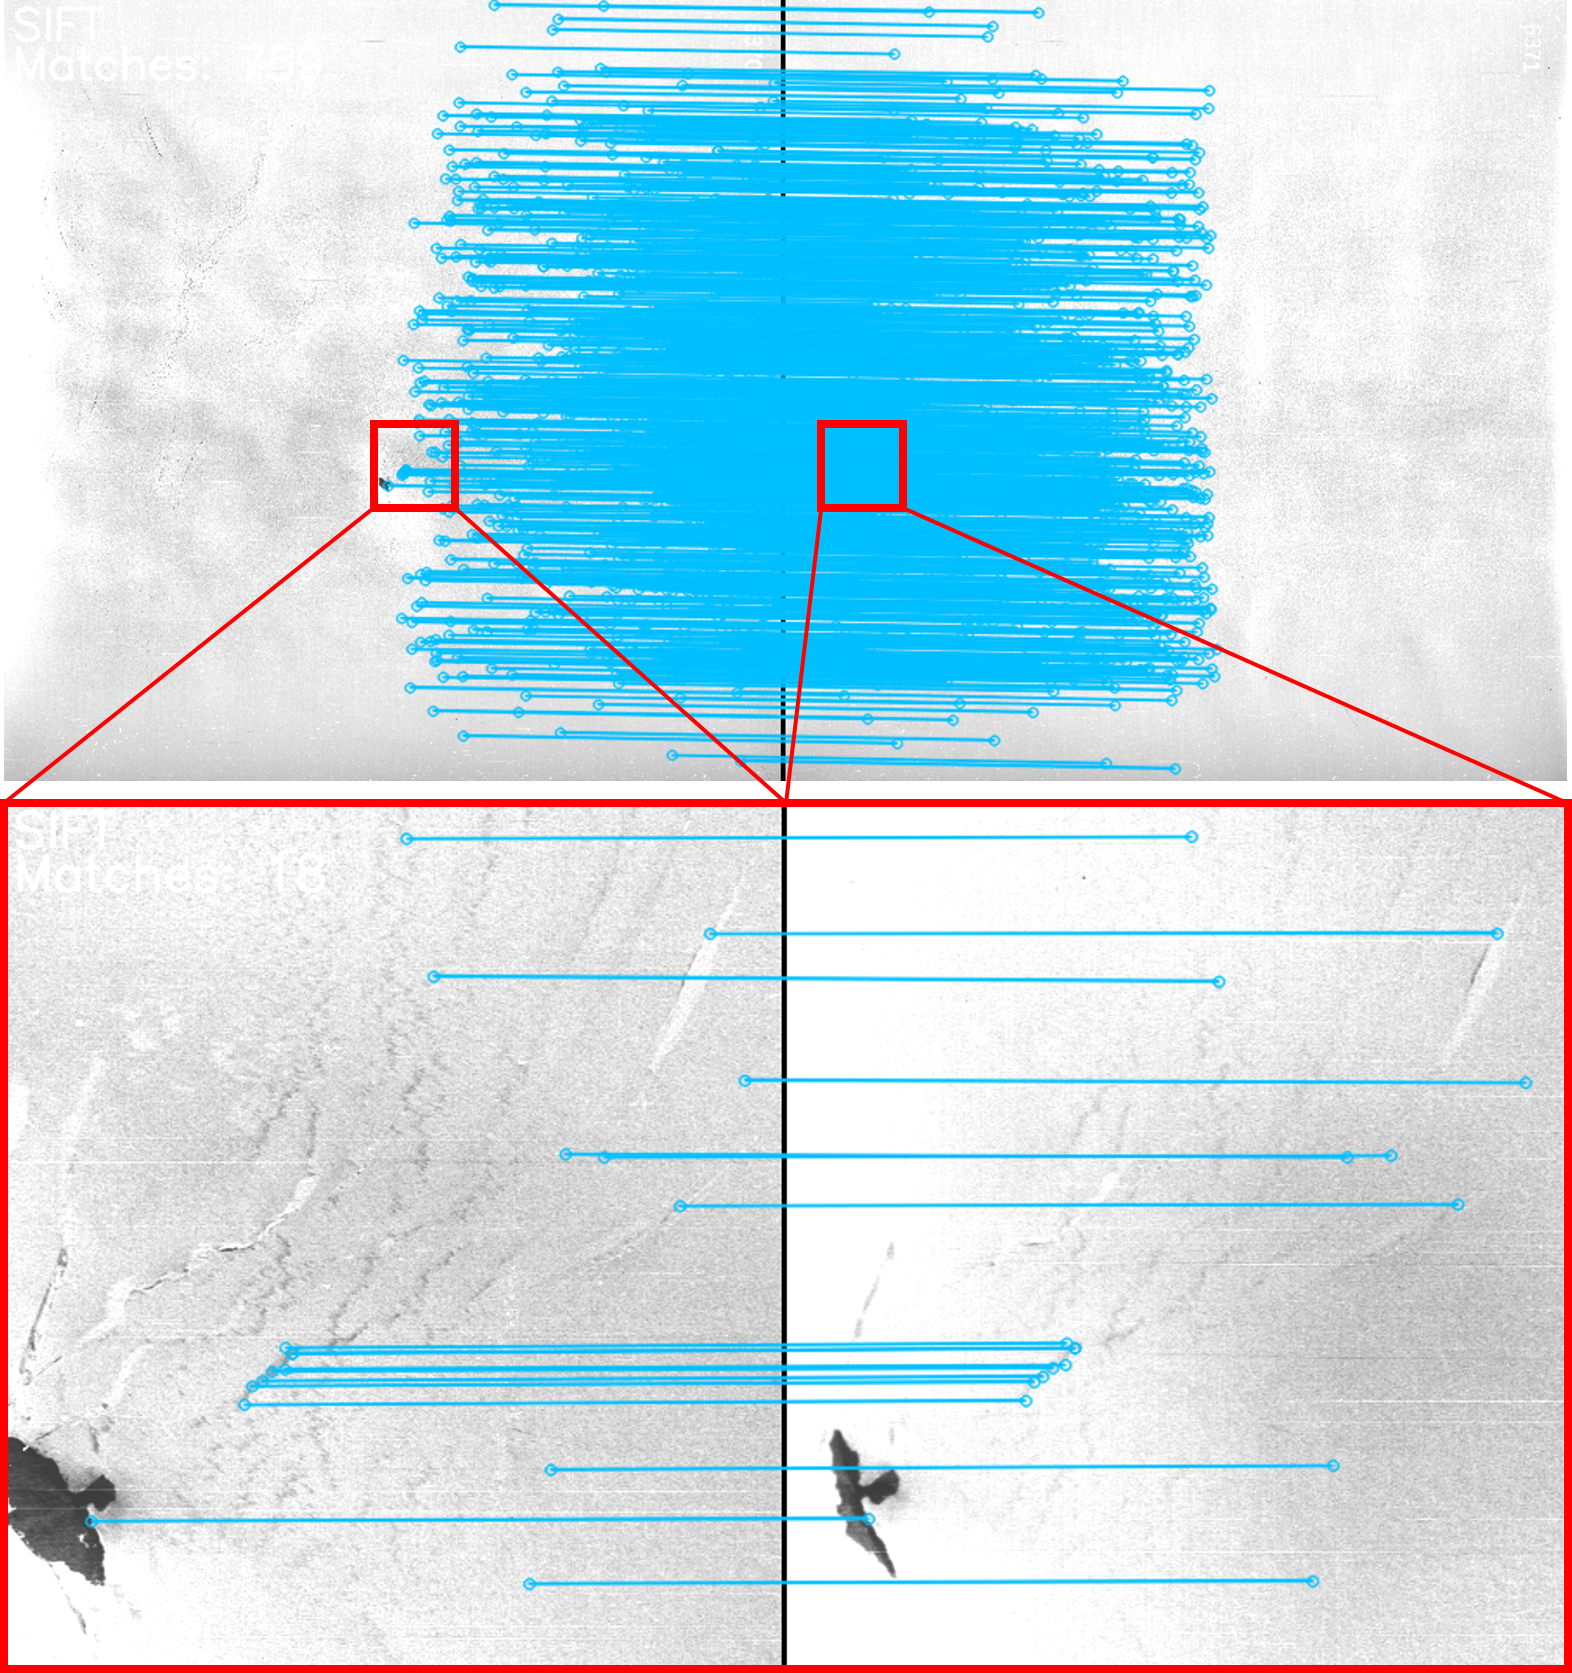
\includegraphics[width=12cm]{images/appendix3/Homol-SIFT2Step-2DRANSAC_3-6370_crp_8Bits_3-6371_crp_8Bits.png}
			\end{minipage}%
		}
		\caption{Matching result of image pair from Figure~\ref{SnowData} (e) and (f). (a) and (b) are matches recovered by SIFT and SuperGlue individually. (c) displayed the matches found by our matching strategy, which is achieved by narrowing down the search space under the guidance of 2D similarity transformation model.}
		\label{Matchresult}
	\end{center}
\end{figure*} 
